\chapter{Reference}

\section{Operations}\label{operations}


\subsection{add +}\label{Operation:add} Add multiple numbers together. The input
  ports allow multiple wires, which are all summed. If an input port
  is unwired, it is equivalent to setting it to zero.

\subsection{subtract $-$}\label{Operation:subtract} Subtract two numbers. The input
  ports allow multiple wires, which are summed prior to the
  subtraction being carried out. If an input port is unwired, it is
  equivalent to setting it to zero. Note the small `+' and `$-$' signs
  on the input ports indicating which terms are added or subtracted from
  the result.

\subsection{multiply $\times$}\label{Operation:multiply} Multiply numbers with each
  other. The input ports allow multiple wires, which are all
  multiplied together. If an input port is unwired, it is equivalent
  to setting it to one.

\subsection{divide $\div$}\label{Operation:divide} Divide a number by another. The
  input ports allow multiple wires, which are multiplied together
  prior to the division being carried out. If an input port is
  unwired, it is equivalent to setting it to one. Note the small
  `$\times$' and `$\div$' signs indicating which port refers to the
  numerator and which the denominator.

\subsection{log}\label{Operation:log} Take the logarithm of the $x$ input port, to
base $b$. The base $b$ needs to be specified --- if the natural
logarithm is desired ($b=e$), use the \htmlref{ln operator}{Operation:ln} instead.

\subsection{pow $x^y$}\label{Operation:pow} Raise one number to the power of another. The
ports are labelled $x$ and $y$, referring the the formula $x^y$.

\subsection{lt $<$}\label{Operation:lt} Returns 0 or 1, depending
  on whether $x<y$ is true (1) or false (0).

\subsection{le $\le$}\label{Operation:le} Returns 0 or 1, depending
  on whether $x\le y$ is true (1) or false (0).

\subsection{eq $=$}\label{Operation:eq} Returns 0 or 1, depending
  on whether $x=y$ is true (1) or false (0).

\subsection{min}\label{Operation:min} Returns the minimum of $x$ and $y$.

\subsection{max}\label{Operation:max} Returns the maximum of $x$ and $y$.

\subsection{and $\wedge$}\label{Operation:and_} Logical and of $x$ and $y$, where
  $x\le 0.5$
  means false, and $x>0.5$ means true. The output is 1 or 0, depending
  on the result being true (1) or false (0) respectively.

\subsection{or $\vee$}\label{Operation:or_} Logical or of $x$ and $y$, where $x\le0.5$
  means false, and $x>0.5$ means true. The output is 1 or 0, depending
  on the result being true (1) or false (0) respectively.

\subsection{not $\neg$}\label{Operation:not_} The output is 1 or 0, depending
  on whether $x\le0.5$ is true (1) or false (0) respectively.

\subsection{time $t$}\label{Operation:time}  Returns the current value of system time.

\subsection{differentiate $d/dt$}\label{Operation:differentiate}
Symbolically differentiates its input.

\subsection{data }\label{Operation:data} \buttonIcon{data.eps} A data interpolation
widget. The data can be imported from a file containing
two values on each line, eg:
\begin{quote}
\begin{tabular}{rr}
0.1 &0.3\\
0.5 &0.7\\
0.9 &1\\
\end{tabular}
\end{quote}

If the input is less than the minimum key value (0.1 here), then the
operation outputs the corresponding value (0.3). Similarly if the
input is greater than the maximum (0.9), the corresponding value (1)
is output. If it lies in between two keys (eg 0.2), the the output is
linearly interpolated (0.4).

Alternatively, the data block can be initialised by a random number
generator, which is a way of introducing random numbers\index{random
  numbers} into the simulation. The parameters are required, the
minimum and maximum values of the function's domain, and the number of
random samples over that domain.

\begin{center}
  \begin{tabular}{cc}
  \resizebox{5.17cm}{!}{\includegraphics{images/initRandom.eps}} &
  \resizebox{0.5\textwidth}{!}{\includegraphics{images/randomExample.eps}}
  \end{tabular}
\end{center}

More formally, a data block is an empirical function, based on a table
of pairs of values ($x_i, y_i, i=1\ldots n, x_{i+1}>x_i$) read in from
a file. The function's output is linearly interpolated from the data,
ie:
\begin{displaymath}
f(x) = \left\{
\begin{array}{cl}
y_1 & x < x_1\\
y_n & x\geq x_n\\
\frac{y_i(x_{i+1}-x)+y_{i+1}(x-x_i)}{x_{i+1}-x_i} & x_i \leq x <
x_{i+1}\\
\end{array}
\right.
\end{displaymath}

\subsection{copy}\label{Operation:copy} This just copies its input to its output,
which is redundant on wiring diagrams, but is needed for internal
purposes.

\subsection{integrate $\int dt$}\label{IntOp}  Creates an integration (or stock)
variable. Editable attributes include the variable's name and its
initial value at $t=0$. The function to be integrated needs to be
connected to the top port. The bottom port can optionally be connected
to a constant, parameter or variable, which is used to specify the
initial value of the integral.

\subsection{sqrt $\surd$}\label{Operation:sqrt} Square root of the input

\subsection{exp}\label{Operation:exp} Exponential of the input

\subsection{ln}\label{Operation:ln} Natural logarithm

\subsection{sin}\label{Operation:sin} sine function
\subsection{cos}\label{Operation:cos} cosine function
\subsection{tan}\label{Operation:tan} tangent function
\subsection{asin}\label{Operation:asin} Arc sine, inverse of sine
\subsection{acos}\label{Operation:acos} Arc cosine, inverse of cosine
\subsection{atan}\label{Operation:atan} Arc tangent, inverse of tangent
\subsection{sinh}\label{Operation:sinh} hyperbolic sine function $\frac{e^x-e^{-x}}2$
\subsection{cosh}\label{Operation:cosh} hyperbolic cosine function $\frac{e^x+e^{-x}}2$
\subsection{tanh}\label{Operation:tanh} hyperbolic tangent function $\frac{e^x-e^{-x}}{e^x+e^{-x}}$
\subsection{abs $|x|$}\label{Operation:abs} absolute value function
\subsection{floor $\lfloor x\rfloor$}\label{Operation:floor} The greatest integer
  less than or equal to $x$.
\subsection{frac}\label{Operation:frac} Fractional part of $x$, ie $x-\lfloor x\rfloor$. 

\section{Tensor operations}\label{tensor operations}\index{tensor|operations}

In the following operations, an axis argument can be supplied in the
operation edit dialog. The axis name is symbolic and available in a
drop down box. If the axis name is not specified, then the operation
will be applied as though the input was flattened (unrolled to a
vector), and then the result reshaped to the original tensor.

\subsection{sum $\sum$}\label{Operation:sum} Sum along a given
axis. 

\subsection{product $\prod$}\label{Operation:product} Multiply along a given axis. 

\subsection{infimum}\label{Operation:infimum} Return the least value
along a given axis. 

\subsection{supremum}\label{Operation:supremum} Return the greatest value
along a given axis. 

\subsection{any}\label{Operation:any} Return 1 if any value
along a given axis is nonzero, otherwise return 0 if all are zero. 

\subsection{all}\label{Operation:all} Return 1 if all values
along a given axis are nonzero, otherwise return 0 if any are zero. 

\subsection{infindex}\label{Operation:infindex} Return the index of
the least value along a given axis.

\subsection{supindex}\label{Operation:supindex} Return the index of
the greatest value along a given axis.

\subsection{running sum $\sum+$}\label{Operation:runningSum} Computes
the running sum of the input tensor along a given axis. For example,
the running sum of $(1,2,3,4)$ is $(1,3,6,10)$.

\subsection{running product $\prod+$}
\label{Operation:runningProduct} Computes the running
product of the input tensor along a given axis. For example, the
running product of $(1,2,3,4)$ is $(1,2,6,24)$.

\subsection{difference $\Delta$}\label{Operation:difference}
Computes the nearest neighbour difference along a given direction. The
optional argument can be used to specify the number of neighbours to
skip in computing the differences.

\subsection{inner product $\cdot$}\label{Operation:innerProduct}
Computes
\begin{displaymath}
z_{i_1,\ldots,i_{r_1-1},j_1,\ldots,j_{r_2-1}} =
\sum_k x_{i_1\ldots,\ldots,i_{r_1-1},k}
y_{k,j_1,\ldots,j_{r_2-1}},
\end{displaymath}
where $a$ is the
given axis, and $r_1$ and $r_2$ are the ranks of $x$ an $y$ respectively.


\subsection{outer product $\otimes$}\label{Operation:outerProduct}
Computes $z_{i_1,i_2,\ldots,i_{r_1},j_1,\ldots,j_{r_2}} =
  x_{i_1,,i_2,\ldots,i_{r_1}}y_{j_1,\ldots,j_{r_2}}$.


\section{Switch}\label{SwitchIcon}

 \buttonIcon{switchIcon.eps}
A switch block (also known as a case block, or select in the Fortran
world) is a way of selecting from a range of alternatives according
to the value of the input, effectively defining a piecewise function.

\begin{center}
  \resizebox{\textwidth}{!}{
\includegraphics{images/switch.eps}}
{\em An example switch block with 3 cases}
\end{center}

The default switch has two cases, and can be used to implement an
if/then/else construct. However, because the two cases are 0 and 1,
or false and true, a two case switch statement will naturally appear
``upside down'' to how you might think of an if statement. In other
words, it looks like:

\parbox{\textwidth}{
{\tt if not }{\em condition} {\tt then}\\
 \ldots
{\tt else}\\
\ldots
}

You can add or remove cases through the context menu. 

\section{Variables}\label{Variable:constant}\label{Variable:parameter}
\label{Variable:flow}\label{Variable:integral}\label{Variable:stock}

Variables represent values in a calculation, and come in a number of
varieties:
\begin{description}
\item[Constants] represent an explicit numerical value, and do not
have a name. Their graphical representation shows the actual value of
the constant.
\item[Parameters] are named constants. All instances of a given name
  represent the same value, as with all other named variables, so
  changing the value of one parameter, either through its edit menu,
  or through a slider, will affect all the others of that
  name. Parameters may be \htmlref{imported from a CSV file}{CSV
    import}, which is one way of inserting a tensor into the
  simulation.
\item[Flow variables] have an input port that defines how the value is
to be calculated. Only one flow variable of a given name can have its
input port connected, as they all refer to the same quantity. If no
input ports are connected, then flow variables act just like
parameters.
\item[Integral variables] represent the result of integrating its
input over time  by means of the differential
equation solver. The integrand is represented by the input to an
integral operator that is attached to the integral variable.
\item[Stock variables] are the columns of Godley tables, and represent
the integral over time of the sum of the flow variables making up the
column.
\end{description}

Variables may be converted between types in the variable edit menu,
available from the context menu, subject to certain rules. For example,
a variable whose input is wired anywhere on the canvas cannot be
changed from ``flow''. Stock variables need to be defined in a Godley
table, and so on.

\subsection{Variable names}

Variable names uniquely identify variables. Multiple icons on the
canvas may have the same name --- they all refer to the same
variable. Variable names have scope, which is either local (no initial
`:'), belonging to an outer \htmlref{group}{Group} (indicated by a leading `:' on the
inner group variable, and the outer group variable having no such
leading `:'), or completely global otherwise. You may select a
variable name from a drop down list in the ``name'' combo box, which
makes for an easier way of selecting exactly which variable you want.

\subsection{Initial conditions}\label{var:init}\index{initial conditions}

Variable initial conditions can be defined through the ``init value''
field of the variable edit menu, or in the case of Godley table stock
variables, through the initial condition row of the Godley table. An
initial value can be a simple number, or it can be a multiple of
another named variable (or parameter). In case of symbolic
definitions, it would be possible to set up a circular reference where
the initial value of variable A is defined in terms of the initial
value of variable B, which in turn depends on the intial value of
A. Such a pathological situation is detected when the system is reset.

\subsection{Tensor valued initial conditions}\label{tensor-init}\index{initial conditions|tensor}

There is also a simple functional language, which allows for the
generation of tensor-valued operations. These functions take the form
{\em func}$(n_1,n_2,\ldots,n_r)$ where $r$ is the desired rank, and
$n_1,n_2,$ etc are the dimensions of the tensor. Available
functions include:

\begin{tabular}{|r|l|}
  \hline
  name & description\\\hline
  \verb+one+ & the tensor is filled with `1'\\
  \verb+zero+ & the tensor is filled with `0'\\
  \verb+iota+ & the arithmetic sequence $(0,1,...\prod_in_i)$\\
  \verb+eye+ & diagonal elements filled with `1', offdiagonal `0'\\
  \verb+rand+ & tensor filled with random numbers in the range $[0,1)$\\
  \hline
\end{tabular}
\index{one}\index{zero}\index{iota}\index{eye}\index{rand}

\begin{itemize}
\item \verb+eye+ is equivalent to \verb+one+ for vectors.
\item \verb+rand+ generates different random numbers each time the simulation
  is reset, and uses the clib \verb+rand()+ function.
\end{itemize}


\subsection{Sliders}

From the context menu, one can select a slider to be attached to a
variable, which is a GUI ``knob'' allowing one to control a variable's
initial value, or the value of a parameter or constant. Adjusting the
slider of an integral (or stock) variable while the system is running
actually adjusts the present value of the variable.

Slider parameters are specified in the edit menu: max, min and step
size. A relative slider means that the step size is expressed as a
fraction of max-min.

\subsection{Importing a parameter from a CSV file}\label{CSV
  import}\index{CSV|import}

After creating a parameter from the ``Variable'' drop-down in the
``Insert'' menu, right-clicking the parameter and selecting the option
to ``Import CSV'', will open a dialogue box that allows you to select 
a CSV file. Upon selecting the file, a dialog is opened, allowing you to 
specify assorted encoding parameters. The dialog looks somewhat like this:

\begin{center}
\resizebox{\textwidth}{!}{\includegraphics{images/CSVimportDialog.eps}}
\end{center}

In this case, the system has automatically guessed that the data is 3
dimensional, and that the first 3 columns give the axis labels for
each dimension (shown in blue), and the 4th column contains the
data. The first row has been automatically determined to be the first
row of the file --- with the dimension names are shown in green.

In this case, the automatic parsing system has worked things out
correctly, but often times it needs help from the computer user. An
example is as follows:

\begin{center}
\resizebox{\textwidth}{!}{\includegraphics{images/CSVimportDialogFail.eps}}
\end{center}

In this example, Minsky has failed to determine where the data starts,
probably because of the ``Unit'' and ``Frequency'' columns. So the first
thing to do is tell it where the data is located by clicking on the
first cell of the data region. 

\begin{center}
\resizebox{\textwidth}{!}{\includegraphics{images/CSVimportDialogSelectData.eps}}
\end{center}

Note that the data region must lie in the bottom right corner of the
table, so you might need to rearrange the CSV file using a speadsheet
program to ensure this. The ``columnar'' option exists as a way of
ignoring any data to the right of a single data column, useful for the
case where some free form comments are appended to the rows.

Now the axes index labels are rendered in blue, the axes names in
green and the data is in black. In this example, some axes duplicate
others, in effect the data is a planar slice through the hypercube. We
can remove these axes from the data by deselecting the column using
the checkbox in the ``Dimension'' row. The deselected columns are
rendered in red, indicating data that is commented out:

\begin{center}
\resizebox{\textwidth}{!}{\includegraphics{images/CSVimportDialogAxesDeselected.eps}}
\end{center}

In this example, the axis names has not been correctly
inferred. Whilst, one can manually edit the axis names in the ``Name''
line, a quick shortcut is to drag ``Header'' and drop it on ``Name'':

The Date column is current parsed as strings, which not only will be
sorted incorrectly, but even if the data were in a YYYYMMDD format
which is sorted correctly, will not have a uniform temporal
spacing. It is therefore important to parse the Date column as
temporal data, which is achieved by changing the column type to
``time'', and specifying a format string, which follows strftime
conventions with the addition of a quarter specifier (\verb+%Q+).
\index{strftime format specifier}\label{strftime format specifier}

\begin{center}
\resizebox{\textwidth}{!}{\includegraphics{images/CSVimportDialogTimeFormat.eps}}
\end{center}

\begin{table}
  \begin{tabular}{|c|l|}
    \hline Code & Description \\\hline
    \%d & Day of month in range 01 to 31\\
    \%H & Hour in range 00 to 23\\
    \%m & Month as a decimal number (01 to 12)\\
    \%M & Minute in range 00 to 59\\
    \%Q & Quarter (0=1st January, 1=1st March etc)\\
    \%s & Number of seconds since epoch (1st January 1970)\\
    \%S & Seconds in range 00 to 59 \\
    \%y & Two digit year YY\\
    \%Y & Four digit year YYYY\\
    \%z & numerical timezone offset\\
    \%Z & Timezone name\\
    \%\% & Literal \% character\\
    \hline
  \end{tabular}
  \caption{Table of strftime codes}
  \label{Strftime code}
\end{table}

Strftime formatted string consists of escape codes (with leading \%
characters). All other characters are treated as matching literally
the characters of the input. So to match a date string of the format
YYYY-MM-DD HH:MM:SS+ZZ (ISO format), use a format string
``\verb|%Y-%m-%d %H:%M:%S+%Z|''. Similarly, for quarterly data
expressed like 1972-Q1, use ``\verb+%Y-Q%Q+''. Note that only \%Y and
\%y can be mixed with \%Q (nothing else makes sense anyway).

Even in the current settings, you may still get a message ``exhausted
memory --- try reducing the rank'', or a similar message about hitting
a 20\% of physical memory threshold. In some cases, ``titles''
and ``addresses'' might be pretty much unique for each record, leading to a
large, but very sparse hypercube. If you remove those columns, as per

\begin{center}
\resizebox{\textwidth}{!}{\includegraphics{images/CSVimportDialogRemoved.eps}}
\end{center}

then you may encounter the ``Duplicate key'' message. In this case, we want
to aggregate over these records, which we can do by setting
``Duplicate Key Action'' to sum. After some additional playing around
with dimensions to aggregate over, we can get the data imported.

\begin{center}
\resizebox{\textwidth}{!}{\includegraphics{images/CSVimportDialogFinal.eps}}
\end{center}

\subsection{Duplicate keys}

In a hypercube, data is indexed by a list of indices, collectively
known as a key. The indices may be strings, integers or date/time
values. If more than one value exists in the CSV file for a given key,
Minsky throws a ``Duplicate key'' exception. This exception gives you
the option of writing a report, which is basically a sorted version of
the original CSV file, with the errors listed at the beginning. You
can open this report in a spreadsheet to see if data needs to be
corrected or removed. 

In the case where the data is correct, but there are still duplicate
keys, such as the example in the previous section, the duplicate keys
may be aggregated over by setting the ``Duplicate Key action'' option.

\section{Wires}

Wire represent the flow of values from one operation to the next. To
add a wire to the canvas, click on the output port of an operation or
variable (right hand side of the icon in its initial unrotated
orientation), and then drag it towards an input port (on the left hand
side of an unrotated icon). You can't connect an operator to itself
(that would be a loop, which is not allowed, unless passing through an
integral), nor can an input port have more than one wire
attached, with the exception of $+/-$ and $\times/\div$, where the
multiple wires are summed or multiplied, respectively, and similarly max/min.

Wires can be bent by dragging the blue dots (``handles''). Every time
a handle is dragged out of a straight line with its neighbours, new
handles appear on either side. Handles can be removed by
double-clicking on them.

\section{Tensor values}\index{tensors}

Variables may have tensor values, or sets of data. Different tensors
are sorted by rank. For example, a tensor of rank 0 may appear as a
single number, let's refer to it as ``x''. A tensor of rank 1 may appear
as a sequence of numbers, let's say ``(x x x x)''. Rank 2 means a tensor
appears as a 2D sequence of numbers, for example:

( x x x )
( x x x )
( x x x )

A tensor of rank 3 will appear as a three-dimensional cube,
rank 4 as a four-dimensional hypercube, and so on. Two 
ways of getting tensor values into Minsky are via tensor-valued 
initial conditions (\S\ref{tensor-init}), or by importing a CSV 
file into a parameter (\S\ref{CSV import}). Scalar 
operations are extended to operating elementwise over tensors, 
and a number of operations exist for operating on tensors 
(\S\ref{tensor operations}).

When two or more tensors are combined with a binary operation (such 
as addition or multiplication), they must have the same rank. For example,
two tensors of rank 2 can be multiplied together, but a tensor of rank 2 and 
a tensor of rank 3 cannot. They may have differing dimensions, which means
the values within each tensor may not necessarily match up 1-to-1 exactly.
To understand what happens when a given dimension is mismatched requires 
understanding the concept of an x-vector\index{x-vector}.

When Minsky is given tensor values, it sorts the values within each tensor
by corresponding dimensions. For example, a rank 2 tensor would have its
values sorted into two sets of data. This data can be in the form of numbers,
dates (time values), or strings. Minsky will then look at cross-sections of the
datasets in order to process the values within. When the dimensions of two
tensors match up, for example two rank 2 tensors, the corresponding
cross-sections of both tensors should also match up. When they don't, a
weighted interpolation of the corresponding values is taken. This involves
using an x-vector.

An x-vector is a vector of real values,
strings or date/time values, and each dimension of a variable has an
implicit or explicit x-vector attached to it. If no x-vector is
explicitly provided, then implicitly it consists of the the values
$(0,\ldots,n_i-1)$, where $n_i$ is the dimension size of axis $i$
of the tensor.

When two tensor values are combined (eg added) along an axis, the
second tensor's value is interpolated according to the
x-vector. Suppose the first tensor was a vector $(x_0,x_1)$ and had an
x-vector (1,3) and the second tensor $(y_0,y_1,y_2)$ had an x-vector
(0,2,3), then the resulting tensor will be $(x_0+0.5(y_0+y_1),
x_1+y_2)$. If the x-vector were date/time data, then the tensor values
will be interpolated according to the actual time values. If the first
tensor's x-vector value lies outside the second tensor's x-vector,
then it doesn't result in a value being included in the output. The
resultant x-vector's range of values is the intersection of input
tensors' x-vector ranges.

If both tensor had string x-vectors, then the resultant tensor will
only have values where both input tensors have the same string value
in their x-vectors. In the above case, where the x-vectors were
('1','3') and ('0','2','3') the resulting tensor will be the scalar $x_1+y_2$.

It goes without saying that the type of the x-vector for each axis
must also match.

\section{Groups}\label{Group}

Grouping gives the capability to create reusable modules, or subroutines that
can dramatically simplify more complicated systems. Groups may be
created in the following ways:
\begin{itemize}
\item by lassoing a number of items to select them, then selecting
``group'' from the canvas context menu, or the edit menu.
\item by pasting the selection. You may ``ungroup'' the group from the
context menu if you don't desire the result of the paste to be a group.
\item by copying another group
\item by inserting a Minsky file as a group
\end{itemize}

Zooming in on a group allows you see and edit its contents. Groups may
be nested heirarchically, which gives an excellent way of zooming in
to see the detail of a model, or zooming out to get an overview of
it. The group context menu item ``Zoom to display'' zooms the canvas
in just enough for the group's contents to be visible.

You may also select ``Open in canvas'' from the context menu. This
replaces the current canvas contents with the contents of the group,
allowing you to edit the contents of the group directly without the
distractions of the rest of the model. Select ``Open master group'' to
return to the toplevel group occupying the canvas.

Around the edges of a group are input or output variables, which allow
one to parameterise the group. One can drag a variable and dock it in
the I/O area to create a new input or output for the group.

When creating a group, or dragging a variable or operation into or out
of a group, if a wire ends up crossing the group boundary, a new
temporary variable is added as an I/O variable.

Variable names within groups are locally scoped to that group. That
means that a variable of the same name outside the group refers to a
different entity completely. One can refer to variables outside the
current scope by prepending the variable name with a `:'. This refers
to a local variable within an outer scope, going all the way to global
scope if no such variable exists. In this way, two groups can share
a variable reference to a variable by using the `:' prefix, and you
can limit the scope of the shared variable by placing a local variable
of the same name in an outer group that both groups are contain within.

A group can also be exported to a file from the context menu.
This allows you to build up a library of building blocks. There is a
github project ``minsky-models'' allowing people to publish their
building blocks and models for others to use. In the future, we hope
to integrate Minsky with this github repository, allowing even more
seamless sharing of models.

\section{Plot widget}
\label{PlotWidget}

A plot widget embeds a dynamic plot into the canvas. Around the
outside of the plot are a number of input ports that can be wired.

\begin{center}

\includegraphics{images/plotWidget.eps}
\end{center}

\begin{description}
\item[left hand edge] Up to 4 quantities can be plotted on the graph
  simultaneously, with line colour given by the colour of the input
  port
\item[right hand edge] Another 4 quantities can be added to the
  plot. These are shown on a different scale to the left hand inputs,
  allowing very different magnitudes to be compared on the one plot.
\item[bottom edge] Quantities controlling the $x$-coordinates of the
  curves. The colours match up with the colour of the pen being
  controlled.

\begin{center}
\includegraphics{images/plotLissajous.eps}
\end{center}

  If only one bottom port is connected, then that controls all pens
  simultaneously, and if no ports are connected, then the simulation
  time is used to provide the $x$ coordinates
\item[corners] Corner ports control the scale. You can wire up
  variables controlling minimum and maximum of the $x$, $y$ and right hand
  $y$ axes. If left unwired, the scales are determined automatically
  from the data. This can be used, for example, to implement a sliding
  window graph

\begin{center}
\includegraphics{images/plotSlidingWindow.eps}
\end{center}
\end{description}

\section{Note Widget}
 \label{Notes}\label{Item} Notes allow arbitrary text to be
placed on the canvas for explanatory purposes. Anything that can be
entered on the keyboard can be placed here, including unicode
characters, and LaTeX formatting is supported. A note
widget, like all canvas items, allow short additional tooltips to be
specified. It is also possible to annotate an ordinary block with some text
that is accessed through the edit menu, or as a tooltip.

\section{Godley Tables}\label{godley}\label{GodleyIcon}

Godley tables describes sets of financial flows from the point of view
of a particular economic agent, such as a bank. The columns of the
table represent accounts (possibly aggregated), which are treated as
integration variables by the system. Accounts may be assets,
liabilities or equities. Assets may appear as liabilities in another
agent's Godley table, and vice versa, with the sense of the financial
flows treated oppositely (a credit flow increasing the asset of one
entity will appear as a debit flow, increasing the value of a
liability). Transfers between accounts should satisfy the {\em
  accounting equation}\index{accounting equation}
(Assets-Liabilities-Equities = 0). So if the transfer is between an
asset and a liability, then it should appear with the same sign (both
positive or both negative), otherwise between two accounts of the same
type, or between a liability and an equity, the terms should have
opposite signs.

Instead of signed flows, one can optionally use CR and DR prefixes, as
specified in the options panel. Each row of the table should have have
one CR entry, and one DR entry. The row sum column should be zero if
it is done correctly.

The first row specifies the stock variables, after which follow the
flow rows. Usually, the row marked ``Initial Conditions'' comes next,
but may be placed in any position. These specify the initial
conditions of the stock variables, and may refer to a multiple of
another variable, just like the \htmlref{initial condition
field}{var:init}, or just be a numerical value.

Finally come the flows. The first column is a simple textual label
(the phrase ``Initial Conditions'', regardless of capitalisation, is a
reserved phrase for setting stock variable initial conditions)
identifying the flow. The flows themselves are written as a numerical
multipler times a flow variable. 

\section{Context Menu}

All canvas items have a context menu, which allow a variety of
operations to be applied to the canvas item. Common context menu items
are explained here:
\begin{description}
\item[Help] bring up context specific help for the item
\item[Description] Attach an annotation to the item. This is only
visible by selecting the description item from the context menu,
although whatever is set as the ``Short Description'' will also appear
as a tooltip whenever the mouse hovers over the item.
\item[Port values] When running a simulation, you can drill down into
the actual values at the input and output ports of the variable or
operation, which is a useful aid for debugging models.
\item[Edit] set or query various attributes of an item. This function
can also be accessed by double clicking on the item. (Plot widgets
behave slightly differently).
\item[Copy] Creates a copy of an item, retaining the same attributes
of the original. This is very useful for creating copies of the same
variable to reduce the amount of overlapping wiring (aka ``rats nest")
in a model.
\item[Flip] actually rotates an object through $180^\circ$. You can
specify aribtrary rotations of objects through the edit menu.
\item[Raise/Lower] Raise and lower the canvas items relative to each
other. You may need to do this if a large item such as a Godley table
or plot is obscuring a wire, making it hard to access the wire's
context menu or handles,
\item[Browse object] gives a low level drilldown of the internal C++
object this canvas item represents. It is perhaps more of interest to
developers. 
\item[Delete] delete the object.
\end{description}

Item specific context menu items:
\begin{description}
\item[variables, parameters and constants]\mbox{}
\begin{description}
\item[Slider] add a slider control to a variable. This is most
effective for controlling parameters and constants, but can also be
used to control inputless variables.
\item[Add integral] attach an integration operation, and convert the
variable into an integral type
\end{description}
\item[integrals]\mbox{}
\begin{description}
\item[Copy Var] copy just the integration variable, not the
integration operation
\item[Toggle Var Binding] Normally, integrals are tightly bound to their
variables. By toggling the binding, the integral icon can then be
moved independently of the variable it is bound to. 
\end{description}
\item[Godley tables]\mbox{}
\begin{description}
\item[Open Godley Table] opens a spreadsheet to allow financial flows
defining the Godley table to be entered or modified.
\item[Resize Godley Table] allows the icon to be resized.
\item[Edit/Copy var] allows individual stock and flow variables to be
copied or edited.
\item[Export to file] export table contents as either CSV data, or as a LaTeX
table, for import into other software.
\end{description}

\item[Groups]\mbox{}
\begin{description}
\item[Zoom to Display] Zoom the canvas sufficiently to see the
contents of the group.
\item[Resize] Resize the group icon on the canvas.
\item[Save group as] Save the group in it's own Minsky file.
\item[Flip contents] Rotate each item within the group by 180$^\circ$
\item[Ungroup] Ungroup the group, leaving it's contents as icons on
the canvas.
\item[contentBounds] Draws a box on the canvas indicating the smallest
bounding box containing the group items.
\end{description}


\item[Plot Widgets]\mbox{}
\begin{description}
\item[Expand]
By double-clicking, or selecting ``Expand'' from the context menu, a
popup window is created of the plot, which can be used examine the
plotting in more detail.

\item[Resize] Allows you to resize the plot icon on the canvas
\item[Options] Customize the plot by adding a title, axes labels and
  control the number of axis ticks and grid lines on the detailed
  plot. You can also add a legend, which is populated from the names
  of variables attached to the plot.
\end{description}

\end{description}

\section{Canvas background}

The canvas is not simply an inert place for the canvas items to
exist. There is also a background context menu, giving access to the
edit menu functionality such as cut/copy/paste, and also keyboard entry.

The following keystrokes insert an operation

\begin{tabular}{rl}
\verb-+- & add\\
\verb+-+ & subtract \\
\verb+*+ & multiply\\
\verb++/ & divide\\
\verb+^+ & pow\\
\verb+&+ & integral\\
\verb+=+ & Godley table\\
\verb+@+ & plot\\
\verb+%+ or \verb+#+ & start a text comment, finish with return\\
\end{tabular}

Typing any other character, then return will insert an operation (if
the name matches), or otherwise a variable with that name.
